% Created 2024-09-15 do. 13:23
% Intended LaTeX compiler: pdflatex
\documentclass[aspectratio=169, usenames,svgnames,dvipsnames]{beamer}
\usepackage[utf8]{inputenc}
\usepackage[T1]{fontenc}
\usepackage{graphicx}
\usepackage{longtable}
\usepackage{wrapfig}
\usepackage{rotating}
\usepackage[normalem]{ulem}
\usepackage{amsmath}
\usepackage{amssymb}
\usepackage{capt-of}
\usepackage{hyperref}
\usepackage{color}
\usepackage{listings}
\usepackage[spanish]{babel}
\setbeamercolor{alerted text}{fg=Blue}
\setbeamerfont{alerted text}{series=\bfseries}
\setbeamercolor{block title}{bg=structure.fg!20!bg!50!bg}
\setbeamercolor{block body}{use=block title,bg=block title.bg}
\AtBeginSubsection[]{\begin{frame}[plain]\tableofcontents[currentsubsection,sectionstyle=show/shaded,subsectionstyle=show/shaded/hide]\end{frame}}
\AtBeginSection[]{\begin{frame}[plain]\tableofcontents[currentsection,hideallsubsections]\end{frame}}
\lstset{keywordstyle=\color{blue}, commentstyle=\color{gray!90}, basicstyle=\ttfamily\small, columns=fullflexible, breaklines=true,linewidth=\textwidth, backgroundcolor=\color{gray!23}, basewidth={0.5em,0.4em}, literate={á}{{\'a}}1 {ñ}{{\~n}}1 {é}{{\'e}}1 {ó}{{\'o}}1 {º}{{\textordmasculine}}1, showstringspaces=false}
\usepackage{mathpazo}
\hypersetup{colorlinks=true, linkcolor=Blue, urlcolor=Blue}
\usepackage{fancyvrb}
\DefineVerbatimEnvironment{verbatim}{Verbatim}{fontsize=\tiny, formatcom = {\color{black!70}}}
\usepackage{pgfplots}
\usetheme{Boadilla}
\usecolortheme{rose}
\usefonttheme{serif}
\author{Francisco Delgado López}
\date{}
\title{Desarrollo de una herramienta software para la simulación de sistemas fotovoltaicos con R}
\subtitle{Trabajo de Fin de Grado}
\institute[UPM]{Universidad Politécnica de Madrid}
\beamertemplatenavigationsymbolsempty
\setbeamertemplate{footline}[frame number]
\setbeamertemplate{itemize items}[triangle]
\setbeamertemplate{enumerate items}[circle]
\setbeamertemplate{section in toc}[circle]
\setbeamertemplate{subsection in toc}[circle]
\hypersetup{
 pdfauthor={Francisco Delgado López},
 pdftitle={Desarrollo de una herramienta software para la simulación de sistemas fotovoltaicos con R},
 pdfkeywords={},
 pdfsubject={},
 pdfcreator={Emacs 29.2 (Org mode 9.6.15)}, 
 pdflang={Spanish}}
\begin{document}

\maketitle

\section{Introducción}
\label{sec:orga0a166c}
\begin{frame}[label={sec:orgd3d4bd1},fragile]{Objetivo principal}
 \begin{block}{Desarrollo de un paquete en \texttt{R}}
\begin{lstlisting}[numbers=left,language=r,label= ,caption= ,captionpos=b]
library(solaR2)
\end{lstlisting}
\end{block}
\end{frame}

\begin{frame}[label={sec:org4f5116e},fragile]{Objetivos secundarios}
 \begin{columns}
\begin{column}{0.2\columnwidth}
\begin{block}{GNU Emacs}
\begin{itemize}
\item \texttt{Org mode}
\item \texttt{ESS}
\end{itemize}
\end{block}
\end{column}
\begin{column}{0.25\columnwidth}
\begin{block}{Paquetes de \texttt{R}}
\begin{itemize}
\item \texttt{solaR}
\item \texttt{zoo}
\item \texttt{data.table}
\item \texttt{microbenchmark}
\item \texttt{profvis}
\item \texttt{lattice}
\end{itemize}
\end{block}
\end{column}
\begin{column}{0.2\columnwidth}
\begin{block}{\LaTeX{}}
\begin{itemize}
\item Documento
\item Presentación
\end{itemize}
\end{block}
\end{column}
\begin{column}{0.25\columnwidth}
\begin{block}{Energía Solar Fotovoltaica}
\begin{center}
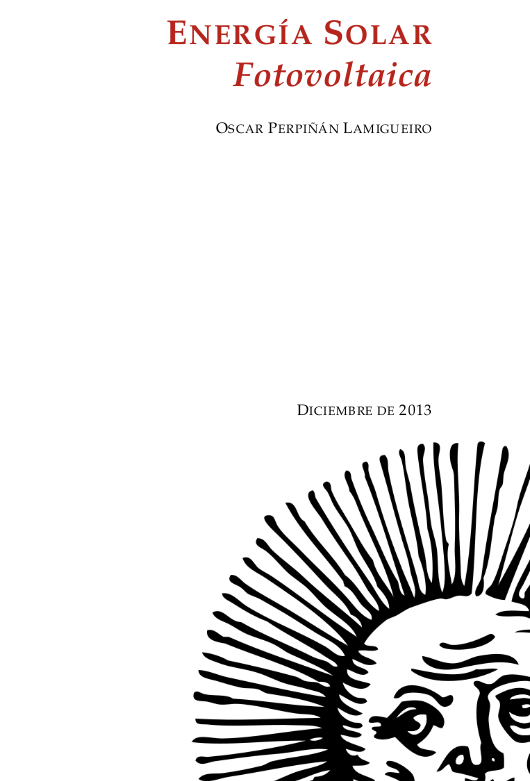
\includegraphics[width=\textwidth]{../figuras/portadaESF.png}
\end{center}
\end{block}
\end{column}
\end{columns}
\end{frame}

\section{Estado del arte}
\label{sec:org6d6ecde}
\subsection{Sitación actual de la generación fotovoltaica}
\label{sec:org7680787}
\begin{enumerate}
\item Crecimiento mundial de la energía fotovoltaica: En 2022, la energía solar fotovoltaica experimentó un crecimiento récord, con 240 GWp de nueva capacidad instalada a nivel mundial, lo que representa un aumento del 137\% respecto a 2021. China lideró este crecimiento, seguida de la Unión Europea, que duplicó su capacidad fotovoltaica.
\item Desarrollo legislativo y de autoconsumo en España: España vivió un auge en el desarrollo fotovoltaico, con un aumento del autoconsumo del 108\% y varias iniciativas legislativas para fomentar las energías renovables y el autoconsumo, como el Plan REPowerEU y medidas para limitar la dependencia del gas.
\item Impacto económico del sector fotovoltaico en España: En 2022, el sector fotovoltaico en España generó un impacto económico significativo, aportando 7.014 millones de euros al PIB y creando 197.383 empleos, consolidando al país como un actor clave en la fabricación y exportación de componentes fotovoltaicos.
\end{enumerate}
\subsection{Soluciones actuales}
\label{sec:org4a73901}
\begin{frame}[label={sec:orgb9f1bfd}]{Soluciones actuales}
\begin{columns}
\begin{column}{0.2\columnwidth}
\begin{block}{\alert{PVsyst}}
\begin{center}

\includegraphics[width=\textwidth]{../figuras/Logo-PVsyst.png}
\end{center}
\end{block}
\end{column}
\begin{column}{0.2\columnwidth}
\begin{block}{\alert{SISIFO}}
\begin{center}

\includegraphics[width=\textwidth]{../figuras/sisifo_naranja_cab2colorpeque1.png}
\end{center}
\end{block}
\end{column}
\begin{column}{0.2\columnwidth}
\begin{block}{\alert{PVGIS}}
\begin{center}

\includegraphics[width=\textwidth]{../figuras/PVGIS.png}
\end{center}
\end{block}
\end{column}
\begin{column}{0.2\columnwidth}
\begin{block}{\alert{System Advisor Model}}
\begin{center}

\includegraphics[width=\textwidth]{../figuras/SAM-logo-horizontal.png}
\end{center}
\end{block}
\end{column}
\end{columns}
\end{frame}
\begin{frame}[label={sec:org2a74c70},fragile]{\texttt{solaR}}
 \begin{columns}
\begin{column}{0.45\columnwidth}
\begin{block}{Funcionamiento}
\begin{itemize}
\item Geometría solar
\item Datos meteorológicos
\item Radiación en el plano horizontal
\item Radiación en el plano del generador
\item Simulación de SFCR
\item Simulación de SFB
\item Optimización de distancias
\item Métodos de visualización
\end{itemize}
\end{block}
\end{column}
\begin{column}{0.45\columnwidth}
\begin{block}{Carencias}
\begin{itemize}
\item Modularidad
\item Eficiencia y rendimiento
\item Escalibilidad
\item Manipulación de datos
\end{itemize}
\end{block}
\end{column}
\end{columns}
\end{frame}

\section{Marco teórico}
\label{sec:org2ce21d3}
\begin{frame}[label={sec:org3bceb74}]{Procedimiento de cálculo}
\begin{center}
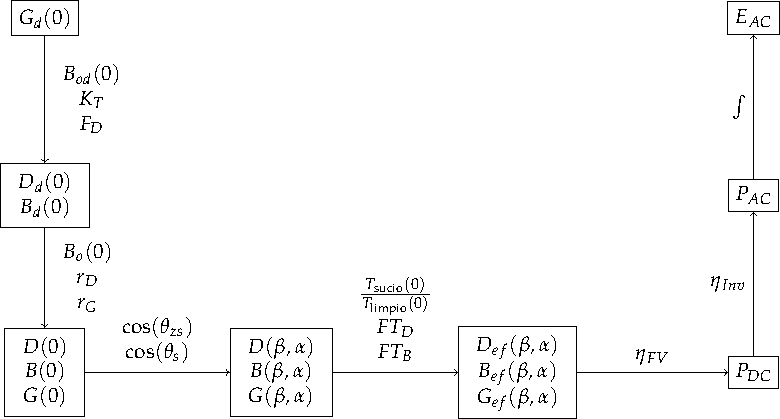
\includegraphics[scale=1]{../figuras/ProcedimientoCalculoRadiacionInclinada.pdf}
\end{center}
\end{frame}
\section{Desarrollo del código}
\label{sec:orgec18bca}
\begin{frame}[label={sec:org4531629}]{Algorítmo de cálculo}
\begin{center}
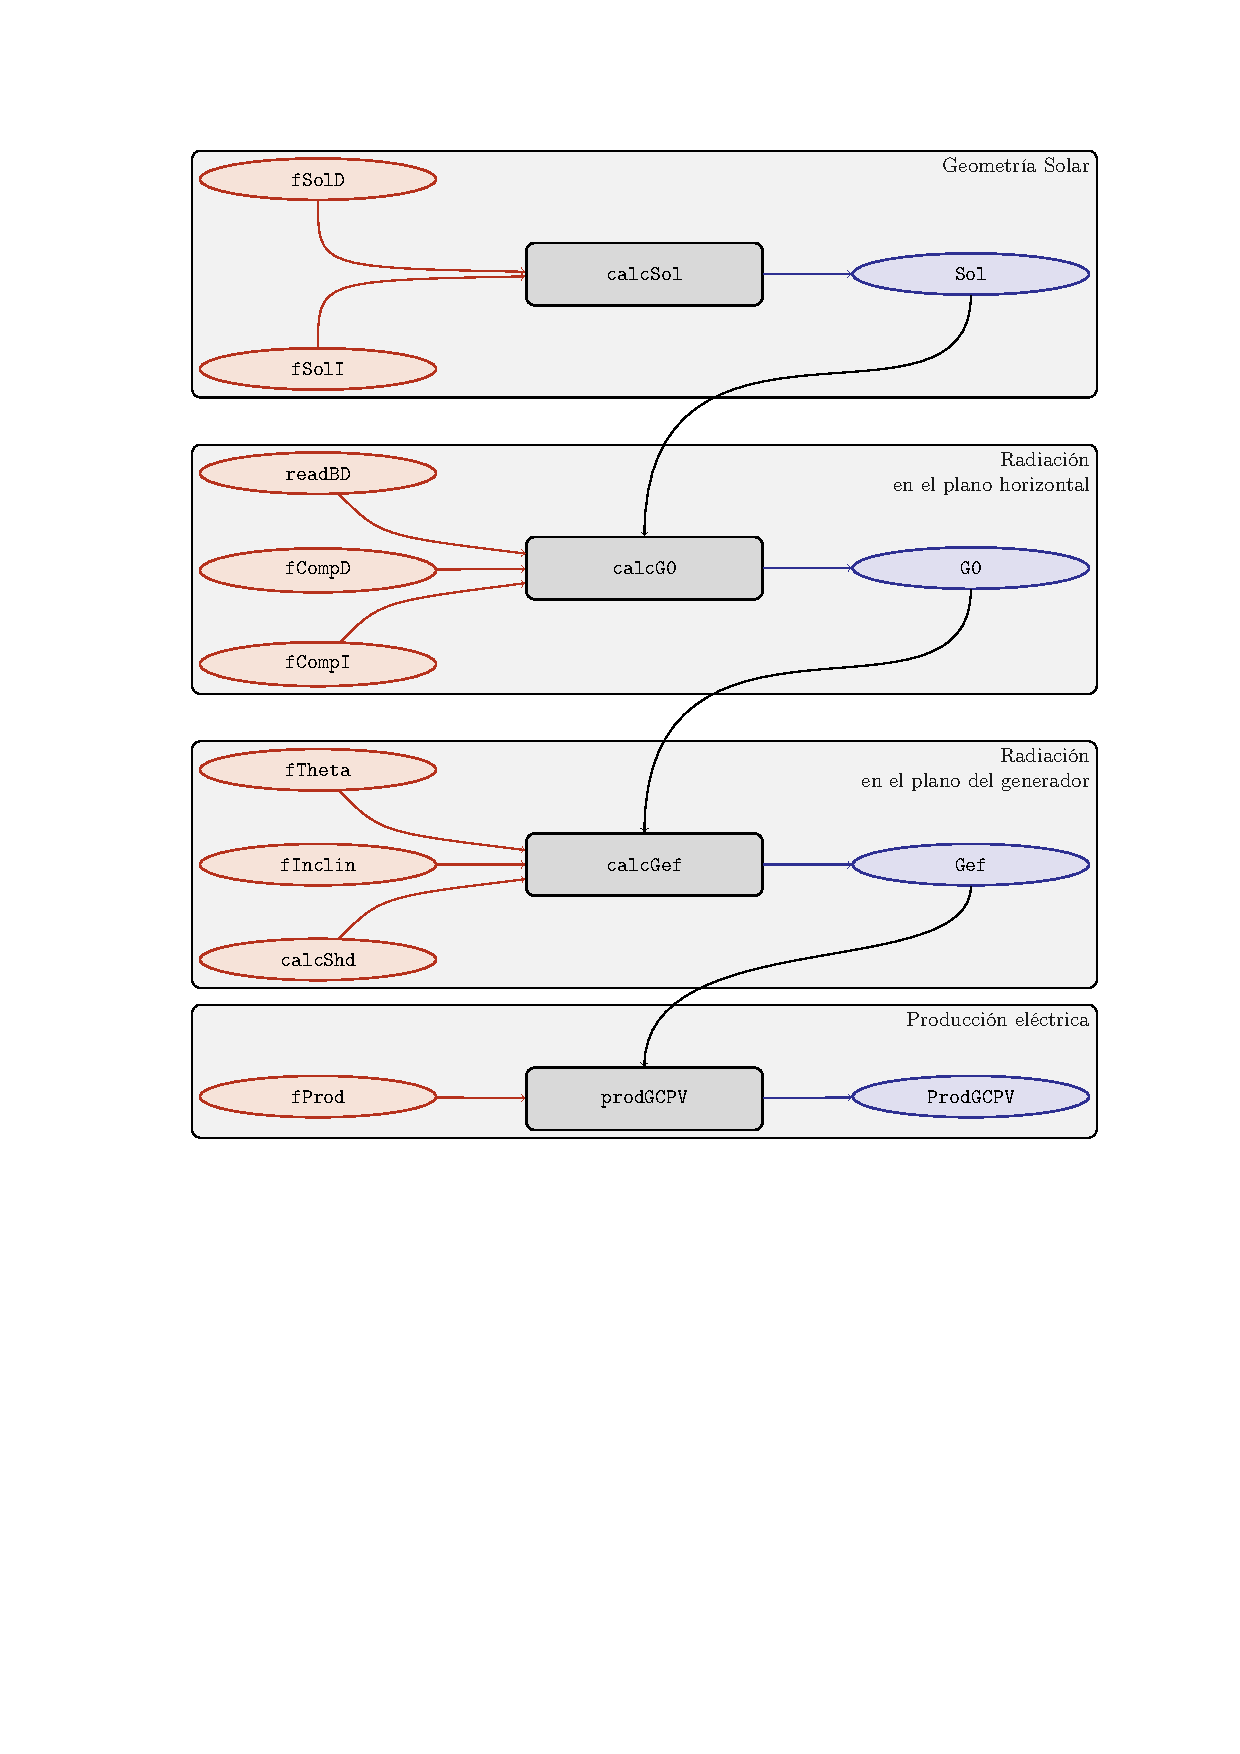
\includegraphics[height=0.9\textheight]{../figuras/procedure.pdf}
\end{center}
\end{frame}
\begin{frame}[label={sec:org35e969f},fragile]{\texttt{calcSol}}
 \begin{center}
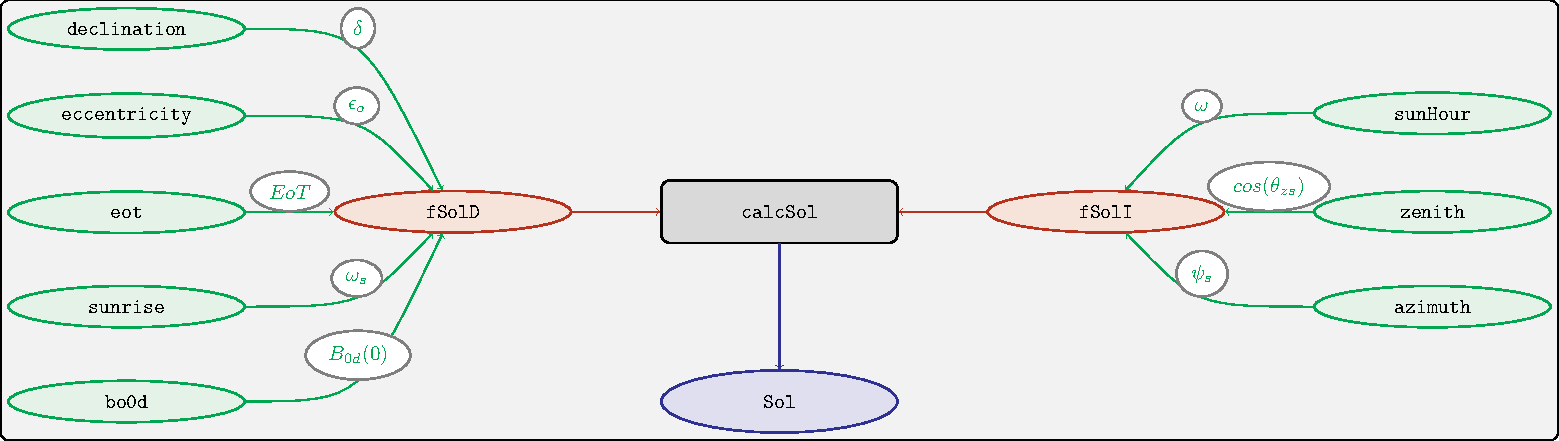
\includegraphics[width=\textwidth]{../figuras/calcsol.pdf}
\end{center}
\end{frame}
\begin{frame}[label={sec:org23eaa72},fragile]{\texttt{Meteo}}
 \begin{center}
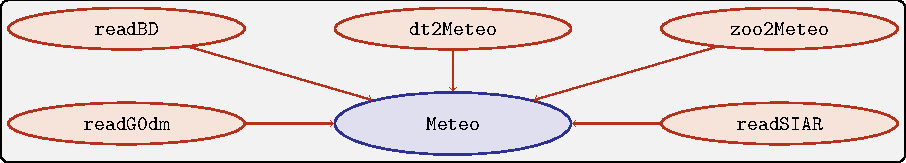
\includegraphics[width=\textwidth]{../figuras/meteo.pdf}
\end{center}
\end{frame}
\begin{frame}[label={sec:org154e5d5},fragile]{\texttt{calcG0}}
 \begin{center}
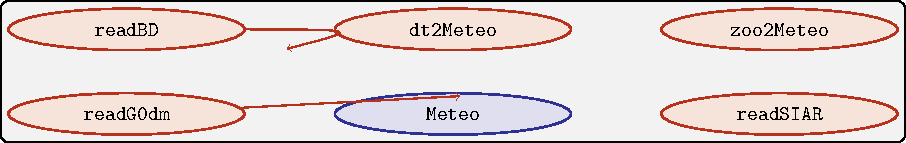
\includegraphics[width=\textwidth]{../figuras/calcg0.pdf}
\end{center}
\end{frame}
\begin{frame}[label={sec:org9c3c817},fragile]{\texttt{calcGef}}
 \begin{center}
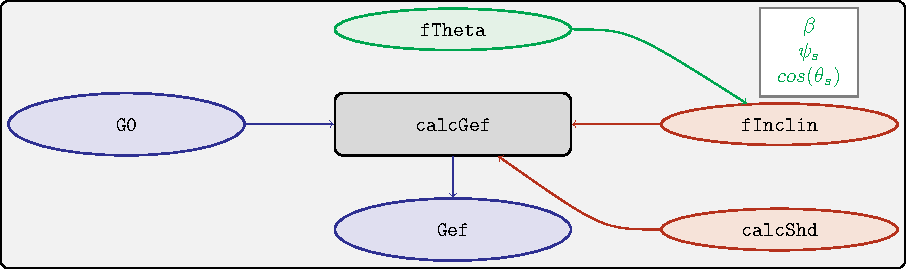
\includegraphics[width=\textwidth]{../figuras/calcgef.pdf}
\end{center}
\end{frame}
\begin{frame}[label={sec:orge6347c9},fragile]{\texttt{prodGCPV}}
 \begin{center}
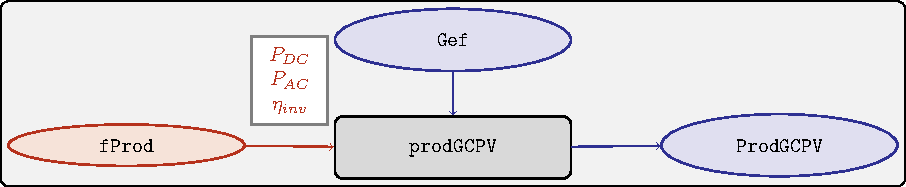
\includegraphics[width=\textwidth]{../figuras/prodgcpv.pdf}
\end{center}
\end{frame}
\begin{frame}[label={sec:orgbdb310c},fragile]{\texttt{prodPVPS}}
 \begin{center}
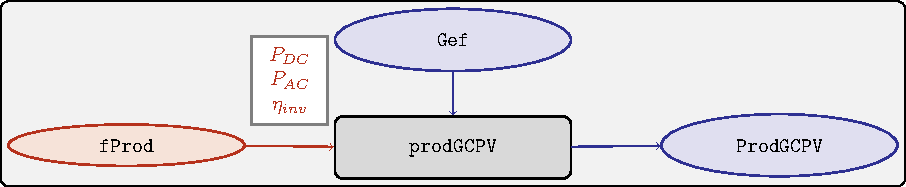
\includegraphics[width=\textwidth]{../figuras/prodpvps.pdf}
\end{center}
\end{frame}
\section{Ejemplo práctico de aplicación}
\label{sec:orgb935394}
\begin{frame}[label={sec:org96bfa1a},fragile]{Información meteorológica}
 \begin{lstlisting}[numbers=left,language=r,label= ,caption= ,captionpos=b]
etsidi_1315 <- readBDi(file = "TFG/data/PVGIS_1315.csv",
                       lat = 40.4, dates.col = "Dates",
                       format = "%Y-%m-%d %H:%M:%S")
\end{lstlisting}

\begin{center}
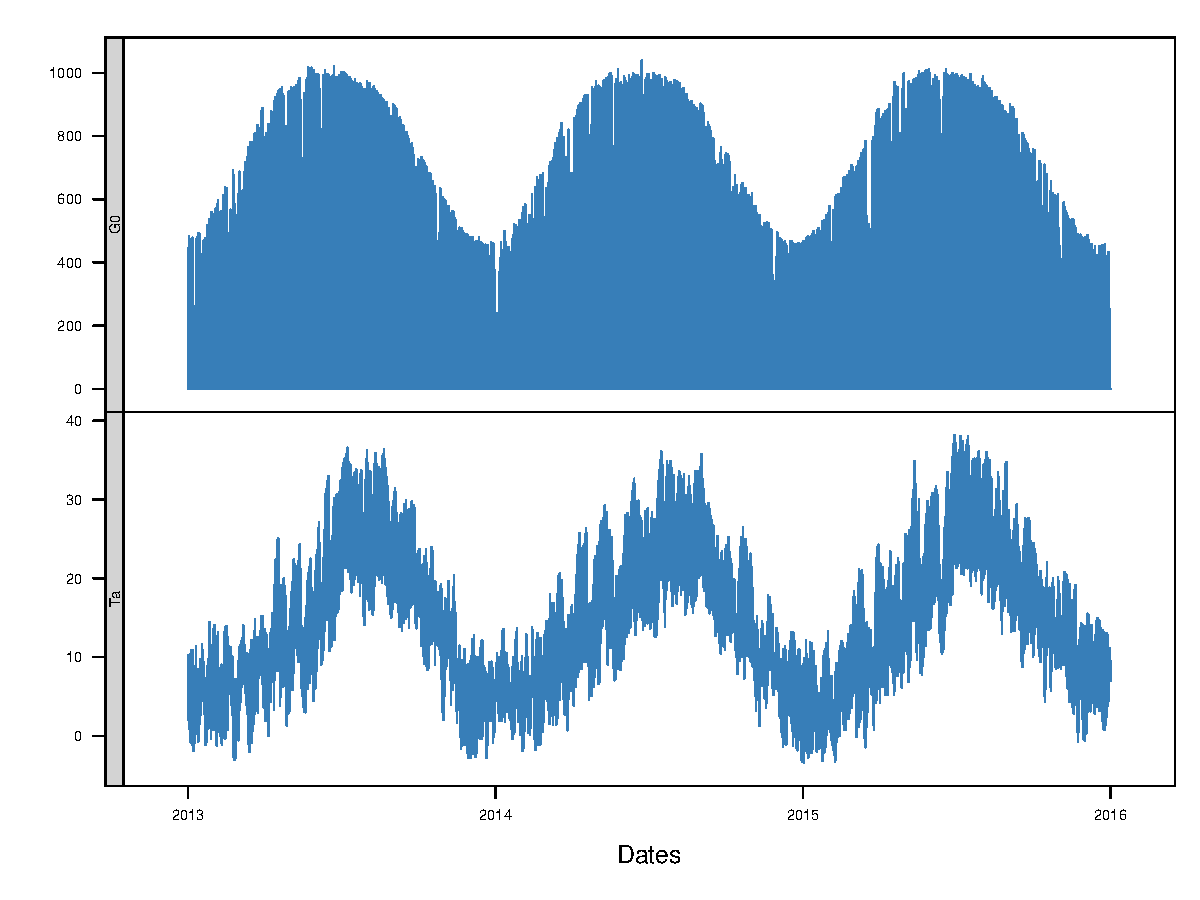
\includegraphics[width=0.5\textwidth]{../figuras/ejemplos3.pdf}
\end{center}
\end{frame}
\begin{frame}[label={sec:org3c397ef},fragile]{Producción de diferentes sistemas}
 \begin{lstlisting}[numbers=left,language=r,label= ,caption= ,captionpos=b]
prod1 <- prodGCPV(lat = 40.4, modeTrk = 'fixed', modeRad = 'bdI',
                  dataRad = etsidi_1315, beta = 30, alpha = -19,
                  module = module1, generator = generator1,
                  inverter = inverter)
show(as.data.tableY(prod1))
\end{lstlisting}

\begin{verbatim}
   Dates      Eac      Edc       Yf
   <int>    <num>    <num>    <num>
1:  2013 1681.077 1757.235 1343.449
2:  2014 1698.613 1775.426 1357.463
3:  2015 1749.536 1828.569 1398.158
\end{verbatim}


\begin{lstlisting}[numbers=left,language=r,label= ,caption= ,captionpos=b]
prod2 <- prodGCPV(lat = 40.4, modeTrk = 'fixed', modeRad = 'bdI',
                  dataRad = etsidi_1315, beta = 30, alpha = -19,
                  module = module2, generator = generator2,
                  inverter = inverter)
show(as.data.tableY(prod2))
\end{lstlisting}

\begin{verbatim}
   Dates      Eac      Edc       Yf
   <int>    <num>    <num>    <num>
1:  2013 1451.873 1517.779 1319.225
2:  2014 1464.483 1530.833 1330.683
3:  2015 1506.544 1574.704 1368.901
\end{verbatim}
\end{frame}

\begin{frame}[label={sec:org411aab1}]{Comparación de producciones}
\begin{center}
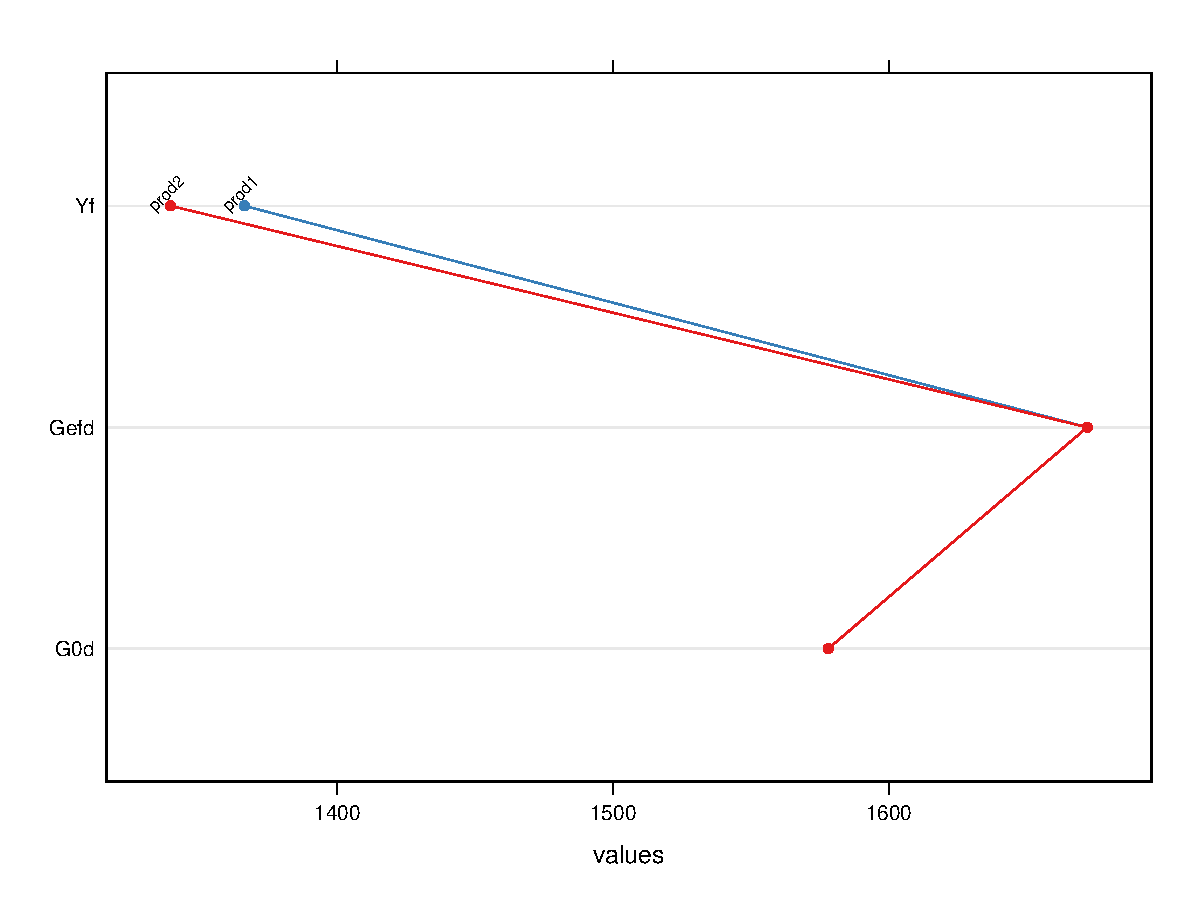
\includegraphics[height=0.9\textheight]{../figuras/ejemplos4.pdf}
\end{center}
\end{frame}
\section{Conclusiones}
\label{sec:orgbbce528}
\subsection{Aportaciones}
\label{sec:orgf64b99b}
\begin{frame}[label={sec:org0f94fc4}]{Blame}
\begin{center}
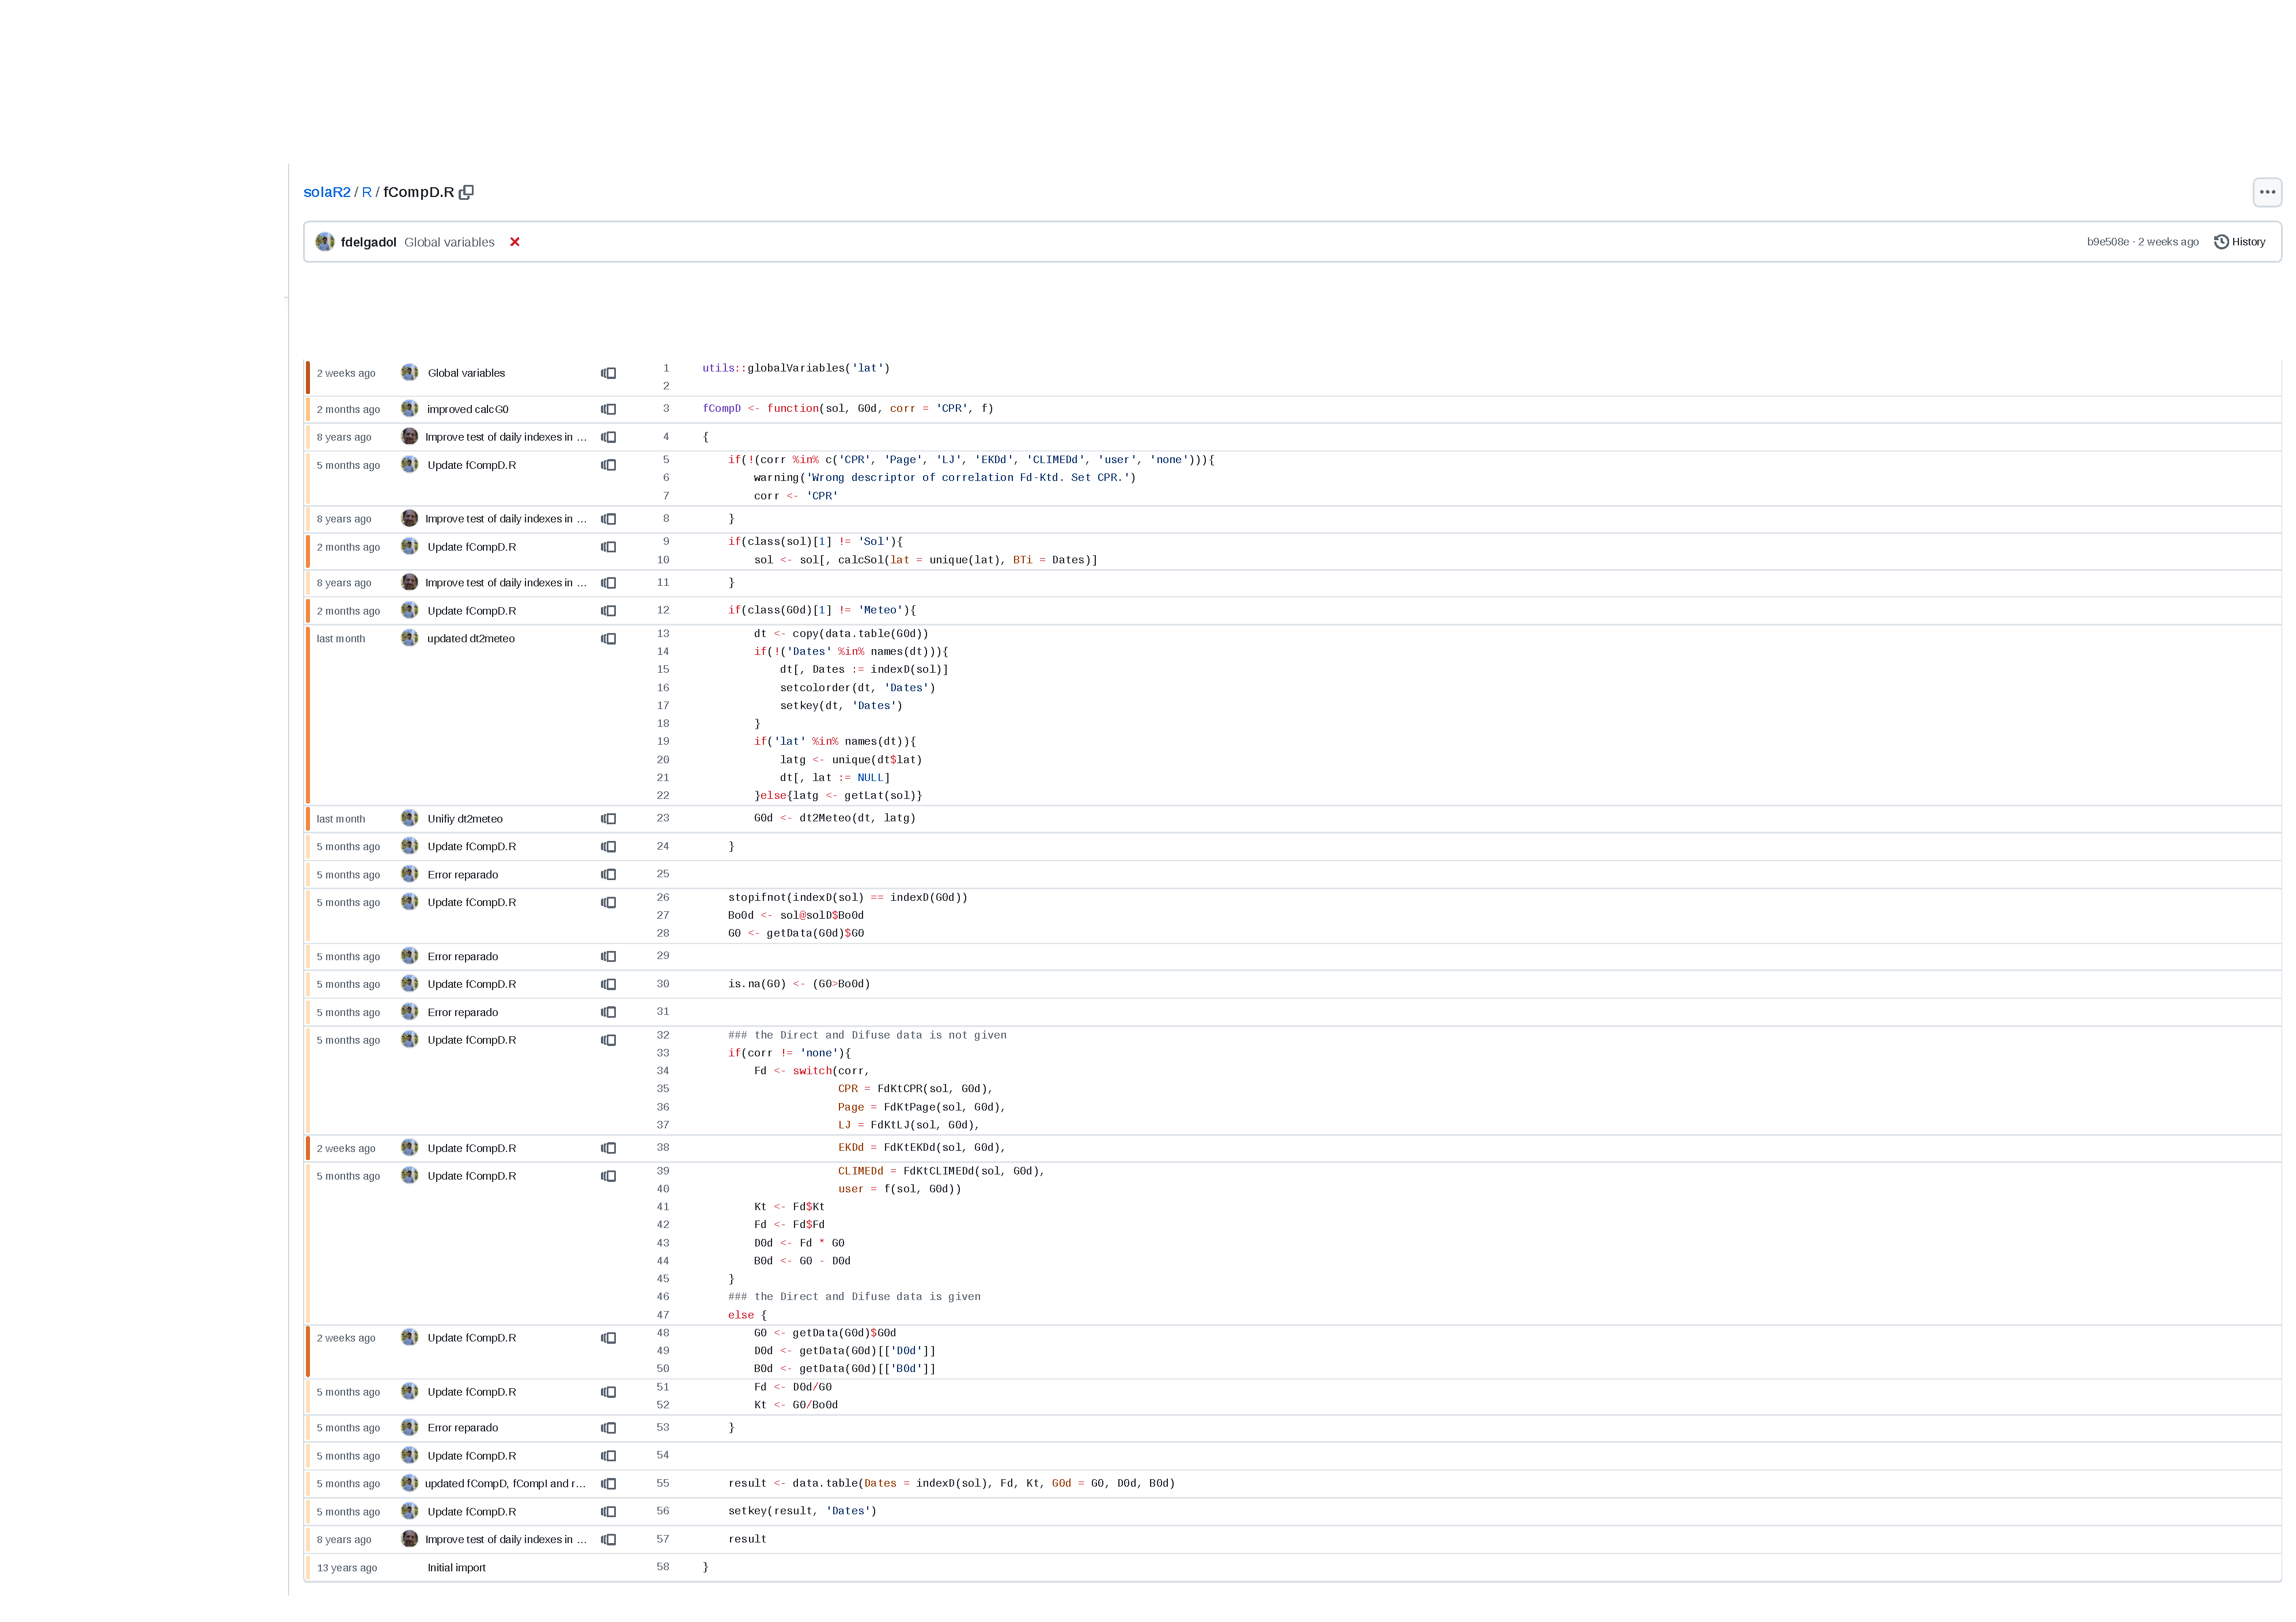
\includegraphics[height=0.9\textheight]{../figuras/blame-fCompD.pdf}
\end{center}
\end{frame}
\begin{frame}[label={sec:org74daa4b}]{Blame}
\begin{center}
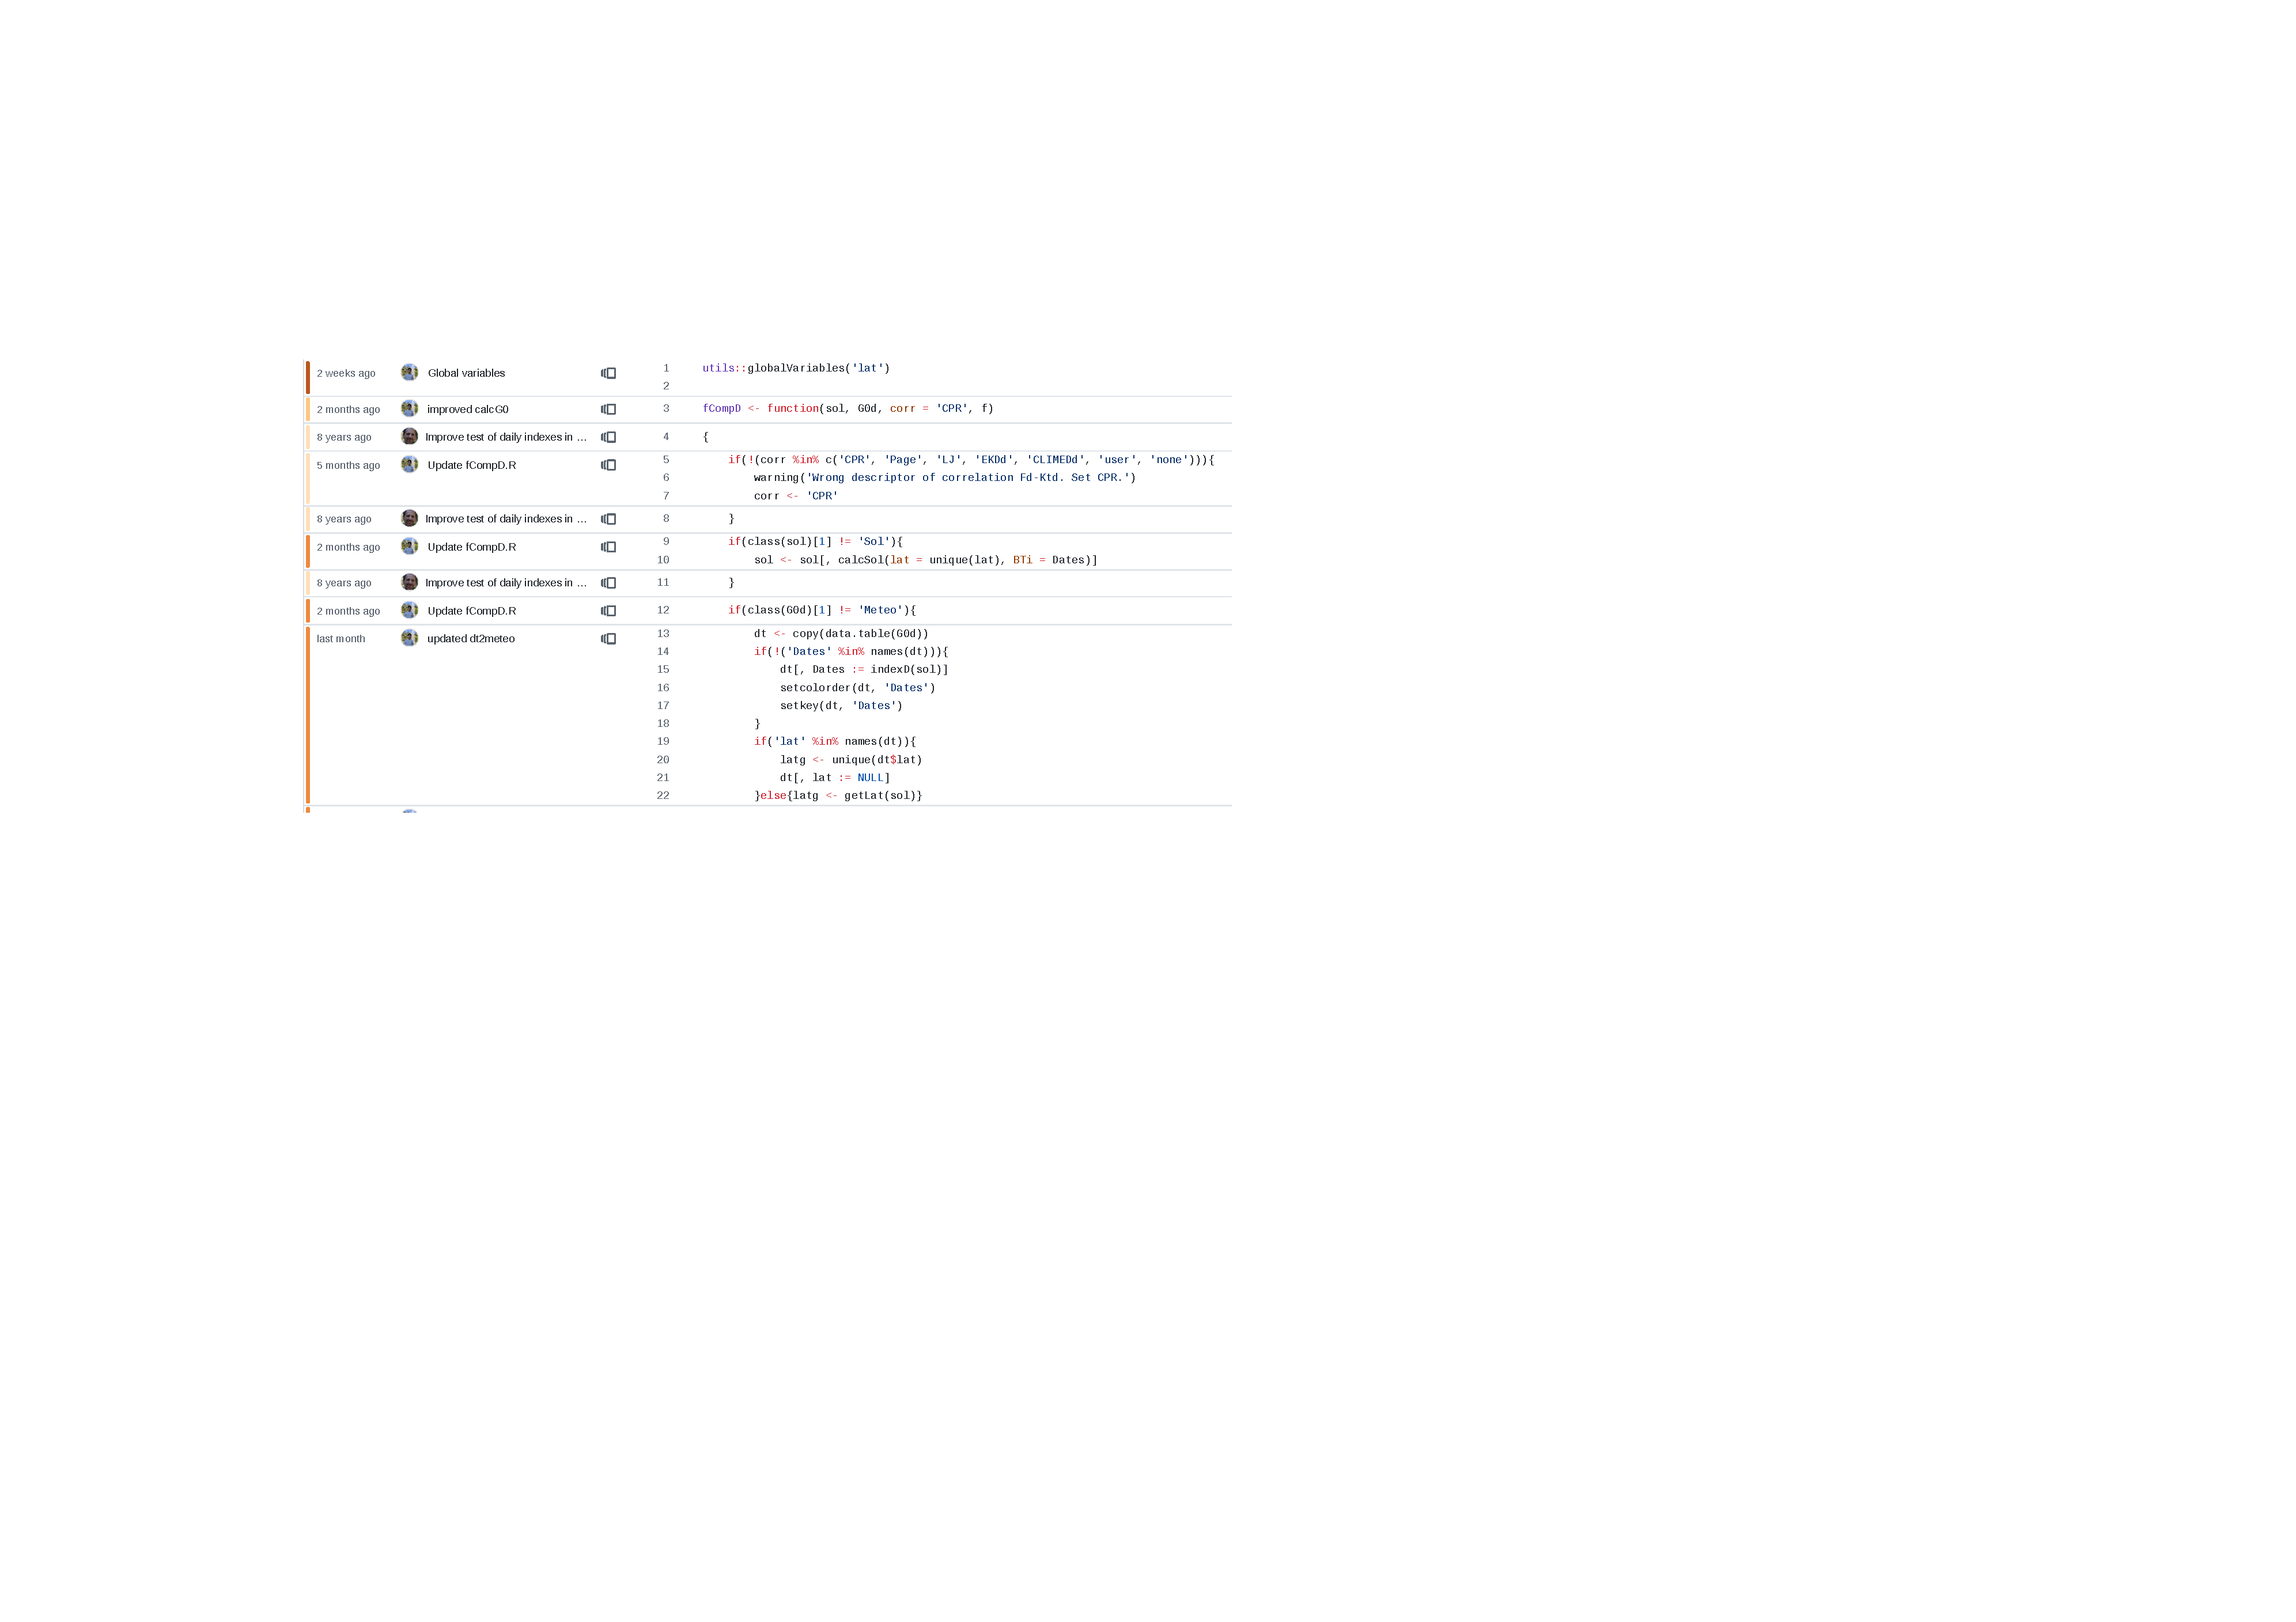
\includegraphics[width=\textwidth]{../figuras/blame-fCompD_cropped.pdf}
\end{center}
\end{frame}
\begin{frame}[label={sec:orgf6e8f7b}]{Insights}
\begin{center}
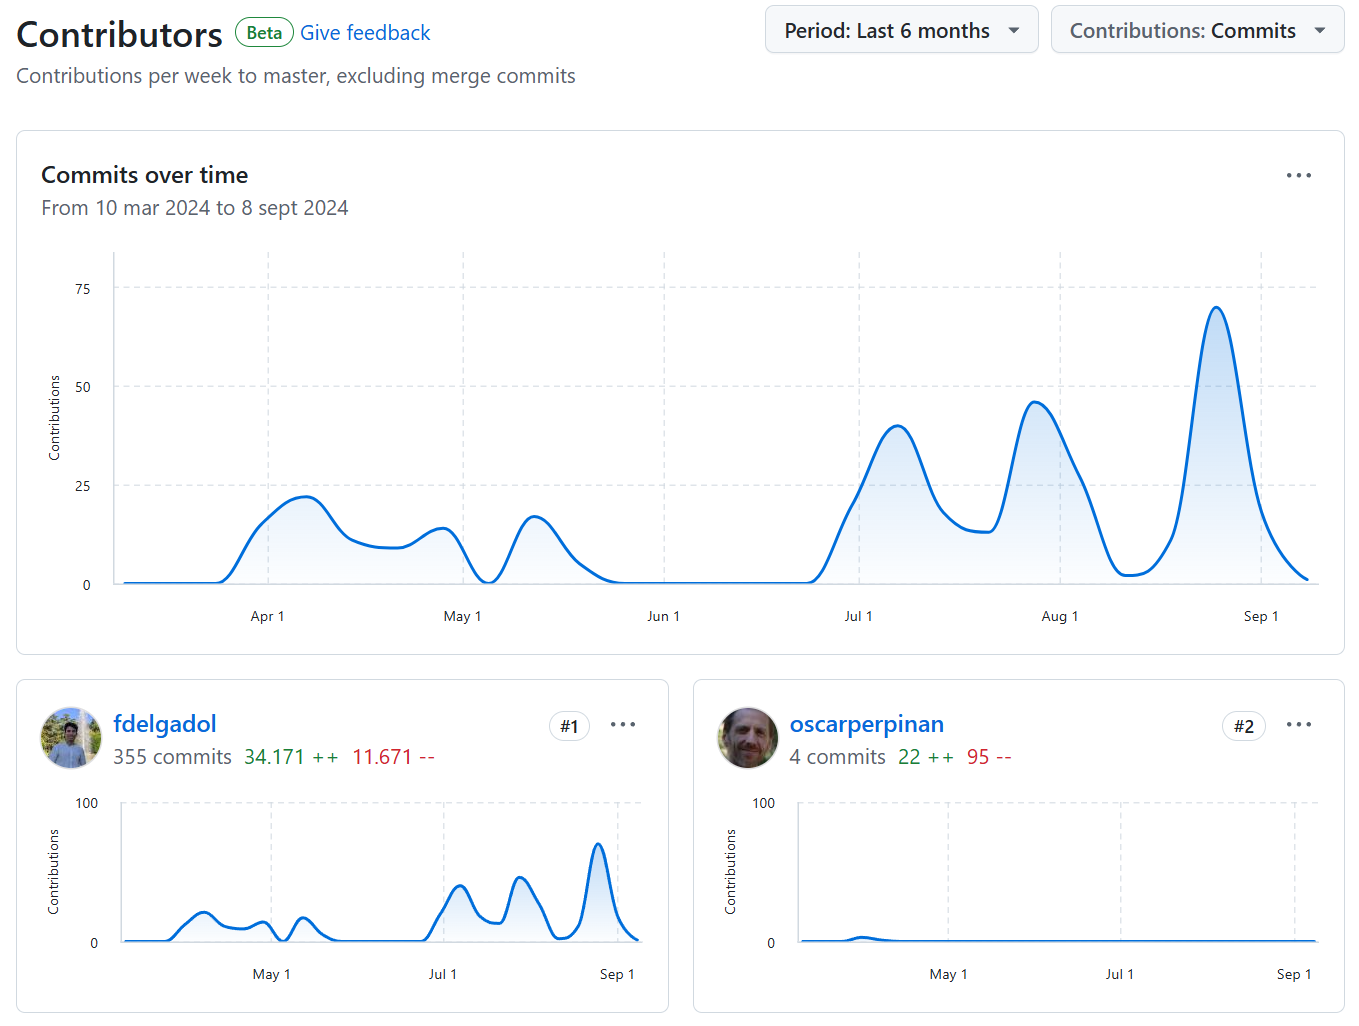
\includegraphics[height=0.9\textheight]{../figuras/contributors.png}
\end{center}
\end{frame}
\subsection{Desarrollo a futuro}
\label{sec:org8fed6e7}
\begin{frame}[label={sec:org362e20a},fragile]{Desarrollo a futuro}
 \begin{block}{Interfaz de usuario}
\end{block}
\begin{block}{Mejora de funciones}
\end{block}
\begin{block}{Toma de datos}
\end{block}
\begin{block}{Uso de paquete especializados en datos espaciales}
\begin{itemize}
\item \texttt{terra}
\end{itemize}
\end{block}
\end{frame}
\end{document}
